\documentclass{article}

\usepackage{url}
\usepackage[hmargin=1.5in]{geometry}
\usepackage{amsmath}
\usepackage{amssymb}
\usepackage{amsthm}
\usepackage{eqnarray}
\usepackage{graphicx}
\usepackage[svgnames]{xcolor} %% for revisions
\usepackage{xparse} %% for squiggly underlines

%%\theoremstyle{definition}
%%\newtheorem{defn}{Definition}
\theoremstyle{plain}
\newtheorem{prop}{Proposition}

% convenience aliases
\newcommand{\maps}{\colon}

% group action
\newcommand{\acts}{\mathbin{\raisebox{\depth}{\rotatebox{-90}{$\circlearrowright$}}}}

% symbology
\newcommand{\Z}{\mathbb{Z}}
\newcommand{\R}{\mathbb{R}}
\newcommand{\C}{\mathbb{C}}
\let\Re\relax
\DeclareMathOperator{\Re}{Re}
\newcommand{\laplace}{\mathcal{L}}
\newcommand{\series}[1]{\tilde{#1}}
\newcommand{\fracderiv}[3]{\partial^{#1}_{#2, #3}}
\newcommand{\holoL}[1]{\mathcal{H}L^{#1}} %% may no longer be needed
\DeclareMathOperator{\Ai}{Ai}

\title{Resurgence of the Airy function}
\author{Aaron Fenyes}

\begin{document}
\maketitle
\section{The Laplace transform}
\subsection{Analytic version}
\subsubsection{Regularity and decay properties}\label{reg-decay}
Let $\zeta$ be the standard coordinate on $\C$, and let $z \maps T^*\C \to \C$ be the fiberwise-linear map $d\zeta \mapsto 1$ (see ``The Geometry of the Laplace Transform'' in {\tt draft2}). The Laplace transform in $\zeta$ turns a function $\varphi$ on $\C$ into a function $\laplace_\zeta \varphi$ on $T^*\C$, defined on the cotangent space of $\zeta = \alpha$ by the integral
\[ \laplace_\zeta \varphi \big|_{\zeta = \alpha} = \int_{\Gamma_{\zeta, \alpha}} e^{-z \zeta}\,\varphi\;d\zeta, \]
where $\Gamma_{\zeta, \alpha}$ is the rightward ray starting at $\zeta = \alpha$ (compare {\tt draft2}). \textcolor{magenta}{We'll use the shorthand $\laplace_{\zeta, \alpha} f := \laplace_\zeta f \big|_{\zeta = \alpha}$ throughout this document [but maybe we should get rid of it].}

Let's say a function $f$ is in $O_{\zeta, \alpha \leftarrow}(g)$ or $O_{\zeta, \alpha \rightarrow}(g)$, respectively, if $|f| \lesssim g$ on some neighborhood of the starting point or infinite end of $\Gamma_{\zeta, \alpha}$. A function is {\em subexponential} along $\Gamma_{\zeta, \alpha}$ if it's in $O_{\zeta, \alpha \rightarrow}(e^{c\zeta})$ for all $c > 0$. Let $\mathcal{E}_{\zeta, \alpha}$ be the space of functions which are subexponential on $\Gamma_{\zeta, \alpha}$, integrable at the starting point, and locally integrable throughout. If $f$ is in $\mathcal{E}_{\zeta, \alpha}$, then $\laplace_{\zeta, \alpha} f$ is well-defined and holomorphic for $\Re(z) > 0$ on the part of $T^*\C$ that lies over $\Gamma_{\zeta, \alpha}$~\cite[\S 5.6]{diverg-resurg-i}.

The asymptotics of $f$ at the starting point of $\Gamma_{\zeta, \alpha}$ control the asymptotics of $\laplace_{\zeta, \alpha} f$ at the infinite end of $\Gamma_{z, 0}$. Once we see how this works for $\alpha = 0$, Section~\ref{translation} will do the rest. Let $F = \laplace_{\zeta, 0} f$. Equation~1.8 of \ref{laplace-tfm} shows\footnote{The argument cited still works in our generality. For holomorphic $f$, one can also use Equation 1.5 of {\em Borel-Laplace Transform and Asymptotic Theory} \textcolor{magenta}{(Sternin \& Shatalov)}.} that
\[ f \in O_{\zeta, 0 \leftarrow}(1) \quad\Longrightarrow\quad F \in O_{z, 0 \rightarrow}\left(\frac{1}{z}\right). \]
More generally, for $\tau > -1$ \textcolor{magenta}{[prove or cite]},
\[ f \in O_{\zeta, 0 \leftarrow}(\zeta^\tau) \quad\Longrightarrow\quad F \in O_{z, 0 \rightarrow}\left(\frac{1}{z^{1 + \tau}}\right). \]
Exact power law asymptotics relate similarly \textcolor{magenta}{[prove or cite]}:
\[ f \sim \zeta^\tau \text{ at the start of } \Gamma_{\zeta, 0} \quad\Longrightarrow\quad F \sim \frac{\Gamma(1+\tau)}{z^{1+\tau}} \text{ at the end of } \Gamma_{z, 0}. \]
\textcolor{magenta}{[The big-$O$ asymptotics dictionary is interesting, but we might not need it. Consider dropping.]}
\subsubsection{Action on integral operators}\label{L-int-op}
When $\varphi \in \mathcal{E}_\zeta$, you can use differentiation under the integral to show that~\cite[Theorem~1.34]{laplace-tfm}
\begin{equation}%%\label{id:L-mult}
\laplace_\zeta (\zeta^n \varphi) = \big({-\tfrac{\partial}{\partial z}}\big)^n \laplace_\zeta \varphi.
\end{equation}
for all integers $n \ge 0$. You can also use a 2d integration argument, akin to the one in \cite[Theorem~2.39]{laplace-tfm}, to show that $\fracderiv{-\lambda}{\zeta}{a} \varphi \in \mathcal{E}_\zeta$ and
\[ \laplace_{\zeta, a}\,\fracderiv{-\lambda}{\zeta}{a} \varphi = z^{-\lambda} \laplace_{\zeta, a} \varphi \]
for all $\lambda \in (0, \infty)$.
\subsection{Change of translation chart}\label{translation}
Define a new coordinate $\zeta_\alpha$ on $\C$ so that $\zeta = \alpha + \zeta_\alpha$. From the calculation
\begin{align*}
\laplace_{\zeta, a} \varphi & = \int_{\Gamma_{\zeta, \alpha}} e^{-z \zeta}\,\varphi\;d\zeta \\
& = \int_{\Gamma_{\zeta_\alpha, 0}} e^{-z(\alpha + \zeta_\alpha)}\,\varphi\;d\zeta_\alpha \\
& = e^{-\alpha z} \int_{\Gamma_{\zeta_\alpha, 0}} e^{-z\zeta_\alpha}\,\varphi\;d\zeta_\alpha \\
& = e^{-\alpha z} \laplace_{\zeta_\alpha, 0} \varphi,
\end{align*}
we learn that
\[ \laplace_{\zeta_\alpha, 0} \varphi = e^{\alpha z} \laplace_{\zeta, \alpha} \varphi. \]
\subsection{Rescaling of translation structure}
Let's rescale the translation structure of $\C$, expanding displacements by a factor of $\mu \in (0, \infty)$. The coordinate $\xi = \mu\zeta$ is a chart for the new translation structure. The corresponding frequency coordinate $x \maps T^*\C \to \C$ is given by $d\xi \mapsto 1$, so $x = \mu^{-1} z$. From the calculation
\begin{align*}
\laplace_{\xi, 0} \varphi & = \int_{\Gamma_{\xi, 0}} e^{-x\xi}\,\varphi\;d\xi \\
& = \int_{\Gamma_{\zeta, 0}} e^{-z \zeta}\,\varphi\;\mu\,d\zeta \\
& = \mu\,\laplace_{\zeta, 0} \varphi
\end{align*}
we learn that
\[ \laplace_{\xi, 0} \varphi = \mu\,\laplace_{\zeta, 0} \varphi. \]
Note that $\laplace_{\xi, 0}$ is defined in the new translation structure on $\C$, while $\laplace_{\zeta, 0}$ is defined in the old translation structure. We can still compare them, because they both turn complex-valued functions on $\C$ into holomorphic functions on $T^*\C$.
\section{Integro-differential equations}
\subsection{Existence of solutions}
\subsubsection{Algebraic integral operators}
Let $D \subset \C$ be an open disk of radius $R$ whose boundary $\partial D$ contains $\zeta = 0$. The Hardy space $H^p(D)$ is the space of holomorphic functions on $D$ which converge pointwise, almost everywhere, to $L^p$ functions on $\partial D$~\cite[Theorem~3.8]{intro-harmonic}. Its norm $\|\cdot\|_p$ is the $L^p$ norm on $\partial D$ with respect to the rotation-invariant probability measure.

We'll study integral operators $\mathcal{G} \acts H^p(D)$ of the form
\[ [\mathcal{G}f](a) = \int_{\zeta = 0}^{a} g(a, \cdot)\,f\,d\zeta, \]
where the kernel $g$ is an algebraic function over $\C^2$ which can be singular on $\Delta$, the diagonal.\footnote{Thanks to Alex Takeda for suggesting this.} To avoid ambiguity, we fix a branch of $g$ to use at the start of the integration path. The domain of $g$ is a covering of $\C^2$ which can be branched over $\Delta$. Continuing $g$ around $\Delta$ changes its phase by a root of unity, leaving its absolute value the same \textbf{[check]}. That makes $|g|$ a well-defined function on $\C^2 \smallsetminus \Delta$, which we can use to bound $\|\mathcal{G}\|$.

\color{SeaGreen}
Assume $p \le q$.

Functions that extend continuously to $\partial D$ are dense in $H^p(D)$ \textcolor{magenta}{[check]}.
\color{black}

\color{DarkBlue}
\begin{align*}
\|\mathcal{G}f\|_1 & = \int_{a \in \partial D} \left| \int_{\zeta = 0}^{a} g(a, \cdot)\,f\,d\zeta \right|\,\frac{|d\zeta(a)|}{2\pi R} \\
& \le \int_{a \in \partial D} \left( \int_{\zeta = 0}^{a} |f|\,|g(a, \cdot)\,d\zeta| \right)\,\frac{|d\zeta(a)|}{2\pi R} \\
& \le \left( \sup_D |f| \right) \int_{a \in \partial D} \left( \int_{\zeta = 0}^{a} |g(a, \cdot)\,d\zeta| \right)\,\frac{|d\zeta(a)|}{2\pi R}.
\end{align*}
By the maximum principle, $\sup_D |f| = \sup_{\partial D} |f|$, so
\[ \|\mathcal{G}f\|_1 \le \|f\|_\infty \int_{a \in \partial D} \left( \int_{\zeta = 0}^{a} |g(a, \cdot)\,d\zeta| \right)\,\frac{|d\zeta(a)|}{2\pi R}. \]
Taking the infimum over all the integration paths we could use to evaluate $[\mathcal{G}f](a)$, we see that
\[ \|\mathcal{G}f\|_1 \le \|f\|_\infty \int_{a \in \partial D} \ell_{g, D}(a)\,\frac{|d\zeta(a)|}{2\pi R}. \]
\color{black}

\begin{align*}
\|\mathcal{G}f\|_p^p & = \int_{a \in \partial D} \left| \int_{\zeta(a') = 0}^{a} g(a, a')\,f(a')\,d\zeta(a') \right|^p\,\frac{|d\zeta(a)|}{2\pi R} \\
& \le \int_{a \in \partial D} \left( \int_{\zeta(a') = 0}^{a} |g(a, a')\,f(a')|\,|d\zeta(a')| \right)^p\,\frac{|d\zeta(a)|}{2\pi R} \\
\end{align*}
Since $\zeta = 0$ and $a$ are both in $\partial D$, and we're assuming that $f$ extends continuously to $\partial D$, we can compute $[\mathcal{G}f](a)$ using an integration path that runs along $\partial D$.
\begin{align*}
\|\mathcal{G}f\|_p^p & \le \int_{a \in \partial D} \left(\int_{a' \in \partial D} |g(a, a')\,f(a')|\,|d\zeta(a')| \right)^p\,\frac{|d\zeta(a)|}{2\pi R} \\
& = \int_{a \in \partial D} \left(2\pi R \int_{a' \in \partial D} |g(a, a')\,f(a')|\,\frac{|d\zeta(a')|}{2\pi R} \right)^p\,\frac{|d\zeta(a)|}{2\pi R} \\
& = (2\pi R)^p \int_{a \in \partial D} \|g(a, \cdot)\,f\|_1^p\;\frac{|d\zeta(a)|}{2\pi R}.
\end{align*}
Then, by H\"{o}lder's inequality,
\begin{align*}
\|\mathcal{G}f\|_p^p & \le (2\pi R)^p \int_{a \in \partial D} \|g(a, \cdot)\|_q^p\;\|f\|_p^p\;\frac{|d\zeta(a)|}{2\pi R} \\
& \le \|f\|_p^p\;(2\pi R)^p \int_{a \in \partial D} \|g(a, \cdot)\|_q^p\;\frac{|d\zeta(a)|}{2\pi R} \\
& \le \|f\|_p^p\;(2\pi R)^p \int_{a \in \partial D} \left( \int_{a' \in \partial D} |g(a, a')|^q\,\frac{|d\zeta(a')|}{2\pi R} \right)^{p/q}\,\frac{|d\zeta(a)|}{2\pi R}.
\end{align*}
Since we're assuming $p \le q$, we can apply Jensen's inequality to the concave function $(\cdot)^{p/q}$ and conclude that
\begin{align*}
\|\mathcal{G}f\|_p^p & \le \|f\|_p^p\;(2\pi R)^p \left( \int_{a \in \partial D} \int_{a' \in \partial D} |g(a, a')|^q\,\frac{|d\zeta(a')|}{2\pi R}\,\frac{|d\zeta(a)|}{2\pi R} \right)^{p/q} \\
& = \|f\|_p^p\;(2\pi R)^p\,\|g\|_q^p,
\end{align*}
which simplifies to
\[ \|\mathcal{G}f\|_p \le \|f\|_p\;2\pi R\,\|g\|_q. \]
That means
\[ \|\mathcal{G}\| \le 2\pi R\,\|g\|_q, \]
where the norm of $g$ is taken with respect to the rotation-invariant probability measure on $(\partial D)^2$.

\color{DarkBlue}
\subsubsection{Algebraic integral operators}
Take a simply connected open set $\Omega \subset \C$ that touches but doesn't contain $\zeta = 0$. Let $\holoL{\infty}(\Omega)$ be the space of bounded holomorphic functions on $\Omega$ with the supremum norm $\|\cdot\|_\infty$. Multiplying by $\zeta^{-\sigma}$ maps $\holoL{\infty}(\Omega)$ isomorphically onto another space of holomorphic functions on $\Omega$. We'll call this space $\holoL{\infty, \sigma}(\Omega)$ and give it the norm $\|f\|_{\infty, \sigma} = \|\zeta^\sigma f\|_\infty$, so that
\begin{align*}
\holoL{\infty}(\Omega) & \to \holoL{\infty, \sigma}(\Omega) \\
\phi & \mapsto \zeta^{-\sigma} \phi
\end{align*}
is an isometry.

%%Let $\mathcal{S} \subset \holoL{\infty}(\Omega)$ be the union of $O_{\zeta, 0 \leftarrow}(\zeta^\tau)$ over all $\tau > 0$.

We'll study integral operators $\mathcal{G} \acts \holoL{\infty, \sigma}(\Omega)$ of the form
\[ [\mathcal{G}f](a) = \int_{\zeta = 0}^{a} g(a, \cdot)\,f\,d\zeta, \]
where the kernel $g$ is an algebraic function over $\C^2$ which can be singular on $\Delta$, the diagonal.\footnote{Thanks to Alex Takeda for suggesting this.} To avoid ambiguity, we fix a branch of $g$ to use at the start of the integration path. The domain of $g$ is a covering of $\C^2$ which can be branched over $\Delta$. Continuing $g$ around $\Delta$ changes its phase by a root of unity, leaving its absolute value the same \textbf{[check]}. That makes $|g|$ a well-defined function on $\C^2 \smallsetminus \Delta$, which we can use to bound $\|\mathcal{G}\|$.

For each $a \in \C$, the expression $|g(a, \cdot)\,d\zeta|$ defines a {\em density} on $\Omega \smallsetminus \{a\}$---a norm on the tangent bundle which is compatible with the conformal structure. The square of a density is a Riemannian metric. Let $\ell_{g, \sigma, \Omega}(a)$ be the distance from $\zeta = 0$ to $a$ with respect to the density $|\zeta(a)^\sigma\,g(a, \cdot)\,\zeta^{-\sigma} d\zeta|$ on $\Omega \smallsetminus \{a\}$. The bound
\begin{align*}
\big|[\zeta^\sigma \mathcal{G}f](a)\big| & \le \left| \zeta(a)^\sigma \int_{\zeta = 0}^{a} g(a, \cdot)\,f\,d\zeta \right| \\
& \le \int_{\zeta = 0}^{a} |\zeta^\sigma f|\,|\zeta(a)^\sigma\,g(a, \cdot)\,\zeta^{-\sigma}\,d\zeta| \\
& \le \|f\|_{\infty, \sigma} \int_{\zeta = 0}^{a} |\zeta(a)^\sigma\,g(a, \cdot)\,\zeta^{-\sigma}\,d\zeta|
\end{align*}
holds for any integration path. Taking the infimum over all paths, we see that
\[ \big|[\mathcal{G}f](a)\big| \le \ell_{g, \sigma, \Omega}(a)\,\|f\|_\infty. \]
so $\|\mathcal{G}\| \le \sup_{a \in \Omega} \ell_{g, \sigma, \Omega}(a)$. Crucially, we can always make $\|\mathcal{G}\|$ a contraction by restricting $\Omega$.
\subsubsection{The example of fractional integrals}
Setting
\[ g(a, a') = \zeta(a)^\rho\,(\zeta(a) - \zeta(a'))^{-\lambda-1}\,\zeta(a')^\mu \]
with $\lambda \in (-\infty, 0)$, we get the operator
\[ \zeta^\rho \circ \partial^\lambda_{\zeta \text{ from } 0} \circ \zeta^\mu. \]
The shortest path from $\zeta = 0$ to $a$ with respect to $|\zeta(a)^\sigma\,g(a, \cdot)\,\zeta^{-\sigma}\,d\zeta|$ is the same as the shortest path with respect to $|d\zeta|$ \textcolor{magenta}{[check]}. It follows that
\begin{align*}
\ell_{g, \sigma, \Omega}(a) & = \int_0^{|\zeta(a)|} |\zeta(a)|^{\rho+\sigma}\,(|\zeta(a)| - r)^{-\lambda-1}\,r^{\mu-\sigma}\,dr \\
& = |\zeta(a)|^{\rho+\sigma} \int_0^1 \,(|\zeta(a)| - |\zeta(a)| t)^{-\lambda-1}\,(|\zeta(a)| t)^{\mu-\sigma}\,|\zeta(a)|\,dt \\
& = |\zeta(a)|^{\rho+\sigma-\lambda-1+\mu-\sigma+1} \int_0^1 \,(1-t)^{-\lambda-1}\,t^{\mu-\sigma}\,dt \\
& = |\zeta(a)|^{\rho-\lambda} \int_0^1 \,(1-t)^{-\lambda-1}\,t^{\mu-\sigma}\,dt \\
& = |\zeta(a)|^{\rho-\lambda+\mu}\,B(-\lambda, \mu-\sigma+1),
\end{align*}
where $B$ is the beta function. Hence, on $\holoL{\infty, \sigma}(\Omega)$,
\[ \|\zeta^\rho \circ \partial^\lambda_{\zeta \text{ from } 0} \circ \zeta^\mu\| \le B(-\lambda,\mu-\sigma+1)\,\sup_\Omega |\zeta|^{\rho-\lambda+\mu}. \]
In particular, when $\Omega$ is small enough that \textcolor{magenta}{[???]}, the operator on the left-hand side is a contraction of $\holoL{\infty, \sigma}(\Omega)$ for all $\lambda \in (-\infty, -\rho]$.
\subsubsection{Fractional integral equations near a regular singular point}
Consider an integral operator $\mathcal{J}$ of the form
\[ p + \partial^{-1}_{\zeta \text{ from } 0} \circ q + \sum_{\lambda \in \Lambda} \partial^\lambda_{\zeta \text{ from } 0} \circ r_\lambda, \]
where:
\begin{itemize}
\item $\Lambda$ is a countable subset of $(-\infty, -1)$.
\item $p$, $q$, and $r_\lambda$ are functions in $\holoL{\infty}(\Omega)$ that extend holomorphically over $\zeta = 0$.
\item $p$ has a first-order zero at $\zeta = 0$.
\end{itemize}

\textcolor{Indigo}{We want to solve the equation $\mathcal{J}f = 0$. Let's look for a solution of the form $f = \zeta^{\tau-1}(1 + \tilde{f})$ with $\tau \in (0, \infty)$ and $\tilde{f} \in \holoL{\infty}(\Omega)$.}

Let $p'_0$ and $q_0$ be the values of $\tfrac{\partial}{\partial \zeta} p$ and $q$, respectively, at $\zeta = 0$. Since $p$, $q$, and $r_\lambda$ extend holomorphically over $\zeta = 0$, and $p$ vanishes at $\zeta = 0$, we can write
\begin{alignat*}{2}
p & = p'_0 \zeta &\;+\;& \tilde{p} \zeta^2 \\
q & = q_0 &\;+\;& \tilde{q} \zeta
\end{alignat*}
where $\tilde{p}, \tilde{q} \in \holoL{\infty}(\Omega)$ extend holomorphically over $\zeta = 0$ too. Then we have
\begin{align*}
\mathcal{J} & = (p_0'\zeta + \tilde{p}\zeta^2) + (q_0\,\partial^{-1}_{\zeta \text{ from } 0} + \partial^{-1}_{\zeta \text{ from } 0} \circ \zeta \circ \tilde{q}) + \sum_{\lambda \in \Lambda} \partial^\lambda_{\zeta \text{ from } 0} \circ r_\lambda \\
& = p'_0\zeta + q_0\,\partial^{-1}_{\zeta \text{ from } 0} + \zeta \circ \tilde{\mathcal{J}},
\end{align*}
where
\[ \tilde{\mathcal{J}} = \tilde{p}\zeta + (\zeta^{-1} \circ \partial^{-1}_{\zeta \text{ from } 0} \circ \zeta) \circ \tilde{q} + \sum_{\lambda \in \Lambda} (\zeta^{-1} \circ \partial^\lambda_{\zeta \text{ from } 0}) \circ r_\lambda. \]
For any $\tau \in (0, \infty)$,
\[ \mathcal{J} \zeta^{\tau-1} = (p'_0 + q_0/\tau)\,\zeta^\tau + [\zeta \circ \tilde{\mathcal{J}}]\,\zeta^{\tau-1}. \]
Setting $\tau = -q_o / p'_0$ makes the first term vanish, leaving
\[ \mathcal{J} \zeta^{\tau-1} = [\zeta \circ \tilde{\mathcal{J}}]\,\zeta^{\tau-1}. \]
The equation $\mathcal{J}f = 0$ then becomes
\begin{align*}
\mathcal{J}\zeta^{\tau-1} + \mathcal{J}(\zeta^{\tau-1}\zeta\tilde{f}) & = 0 \\
\tilde{\mathcal{J}}\zeta^{\tau-1} + [\mathcal{J} \circ \zeta](\zeta^{\tau-1}\tilde{f}) & = 0 \\
\end{align*}

\textcolor{DodgerBlue}{We want to solve the equation $\mathcal{J}f = 0$. Let's look for a solution of the form $f = \zeta^{\tau-1} + \tilde{f}$ with $\tau \in (0, \infty)$ and $\tilde{f} \in \holoL{\infty}(\Omega)$.}

\color{SeaGreen}
\begin{prop}\label{prop:frac-mollify}
If $f$ is in $O_{\zeta, 0 \leftarrow}(\zeta^\alpha)$ with $\alpha \in (-1, \infty)$, then $\partial^\lambda_{\zeta \text{ from } 0}\,f$ is in $O_{\zeta, 0 \leftarrow}(\zeta^{\alpha-\lambda})$ for all $\lambda \in (-\infty, 0)$.
\end{prop}
\color{magenta}
\begin{proof}
??????
\end{proof}
\color{SeaGreen}
\begin{prop}\label{prop:frac-int-growth}
For any $f \in \holoL{\infty}(\Omega)$ and $\lambda \in (-\infty, 0)$, the bound
\[ \big|\partial^\lambda_{\zeta \text{ from } 0}\,f\big| \le (-\tfrac{1}{\lambda}) |\zeta|^{-\lambda} \|f\|_\infty \]
holds pointwise throughout $\Omega$.
\end{prop}
\color{magenta}
\begin{proof}
??????
\end{proof}
\color{DodgerBlue}

Let $p'_0$ and $q_0$ be the values of $\tfrac{\partial}{\partial \zeta} p$ and $q$, respectively, at $\zeta = 0$. Since $p$, $q$, and $r_\lambda$ extend holomorphically over $\zeta = 0$, and $p$ vanishes at $\zeta = 0$, we can write
\begin{alignat*}{2}
p & = p'_0 \zeta &\;+\;& \tilde{p} \zeta^2 \\
q & = q_0 &\;+\;& \tilde{q} \zeta \\
\textcolor{orange}{r_\lambda} & = r_{\lambda,0} &\;+\;& \tilde{r}_\lambda \zeta,
\end{alignat*}
where $\tilde{p}, \tilde{q} \in \holoL{\infty}(\Omega)$ extend holomorphically over $\zeta = 0$ too. For any $\tau \in (0, \infty)$,
\begin{align*}
\mathcal{J} \zeta^{\tau-1} & = p'_0 \zeta^\tau + \tilde{p} \zeta^{\tau+1} + \partial^{-1}_{\zeta \text{ from } 0}\big(q_0 \zeta^{\tau-1}\big) + \partial^{-1}_{\zeta \text{ from } 0}\big(\tilde{q} \zeta^\tau\big) + \sum_{\lambda \in \Lambda} \partial^\lambda_{\zeta \text{ from } 0} \big(r_\lambda \zeta^{\tau-1}\big) \\
& = (p'_0 + q_0/\tau)\zeta^\tau + \tilde{p} \zeta^{\tau+1} + \partial^{-1}_{\zeta \text{ from } 0}\big(\tilde{q} \zeta^\tau\big) + \sum_{\lambda \in \Lambda} \partial^\lambda_{\zeta \text{ from } 0} \big(r_\lambda \zeta^{\tau-1}\big).
\end{align*}
Setting $\tau = -q_o / p'_0$ makes the first term vanish, leaving
\begin{align*}
\mathcal{J} \zeta^{\tau-1} & = \textcolor{SeaGreen}{\tilde{p} \zeta^{\tau+1} + \partial^{-1}_{\zeta \text{ from } 0}\big(\tilde{q} \zeta^\tau\big) + \sum_{\lambda \in \Lambda} \partial^\lambda_{\zeta \text{ from } 0} \big(r_\lambda \zeta^{\tau-1}\big).} \\
\mathcal{J} \zeta^{\tau-1} & = \tilde{p} \zeta^{\tau+1} + \partial^{-1}_{\zeta \text{ from } 0}\big(\tilde{q} \zeta^\tau\big) + \sum_{\lambda \in \Lambda} \partial^\lambda_{\zeta \text{ from } 0} \big(r_{\lambda,0} \zeta^{\tau-1} + \tilde{r}_\lambda \zeta^\tau\big) \\
& \textcolor{orange}{= \tilde{p} \zeta^{\tau+1} + \partial^{-1}_{\zeta \text{ from } 0}\big(\tilde{q} \zeta^\tau\big) + \sum_{\lambda \in \Lambda} \left[ r_{\lambda,0} \tfrac{\Gamma(\tau)}{\Gamma(\tau-\lambda)} \zeta^{\tau-1-\lambda} + \partial^\lambda_{\zeta \text{ from } 0} \big(\tilde{r}_\lambda \zeta^\tau\big) \right]} \\
& \textcolor{orange}{= \tilde{p} \zeta^{\tau+1} + \sum_{\lambda \in \Lambda} \left[ r_{\lambda,0} \tfrac{\Gamma(\tau)}{\Gamma(\tau-\lambda)} \zeta^{\tau-(\lambda+1)} \right] + \left[ \partial^{-1}_{\zeta \text{ from } 0} \circ \tilde{q} + \sum_{\lambda \in \Lambda} \partial^\lambda_{\zeta \text{ from } 0} \circ \tilde{r}_\lambda \right] \zeta^\tau.}
\end{align*}
Now we can rewrite the equation $\mathcal{J}(\zeta^{\tau-1} + \tilde{f}) = 0$ as
\begin{align*}
\mathcal{J} \zeta^{\tau-1} + \left[ p + \partial^{-1}_{\zeta \text{ from } 0} \circ q + \sum_{\lambda \in \Lambda} \partial^\lambda_{\zeta \text{ from } 0} \circ r_\lambda \right] \tilde{f} & = 0 \\
\mathcal{J} \zeta^{\tau-1} + \left[ \partial^{-1}_{\zeta \text{ from } 0} \circ q + \sum_{\lambda \in \Lambda} \partial^\lambda_{\zeta \text{ from } 0} \circ r_\lambda \right] \tilde{f} & = -p\tilde{f}.
\end{align*}
Observing that
\[ \frac{1}{p} = \frac{\zeta^{-1}}{p_0 + \tilde{p} \zeta}, \]
we have
\begin{align*}
\frac{1}{p}\,\mathcal{J} \zeta^{\tau-1} & = \frac{1}{p_0 + \tilde{p} \zeta} \left[ \tilde{p} \zeta^\tau + \zeta^{-1}\,\partial^{-1}_{\zeta \text{ from } 0}\big(\tilde{q} \zeta^\tau\big) + \sum_{\lambda \in \Lambda} \left[ r_{\lambda,0} \tfrac{\Gamma(\tau+1)}{\Gamma(\tau-\lambda+1)} \zeta^{\tau-(\lambda+\textcolor{magenta}{2})} + \zeta^{-1}\,\partial^\lambda_{\zeta \text{ from } 0} \big(\tilde{r}_\lambda \zeta^\tau\big) \right] \right] \\
\frac{1}{p}\,\mathcal{J} \zeta^{\tau-1} & = \frac{1}{p_0 + \tilde{p} \zeta} \left[ \tilde{p} \zeta^\tau + \sum_{\lambda \in \Lambda} \left[ r_{\lambda,0} \tfrac{\Gamma(\tau+1)}{\Gamma(\tau-\lambda+1)} \zeta^{\tau-(\lambda+\textcolor{magenta}{2})} \right] \right] + \frac{1}{p_0 + \tilde{p} \zeta} \left[ \zeta^{-1}\,\partial^{-1}_{\zeta \text{ from } 0} \circ \tilde{q} + \sum_{\lambda \in \Lambda} \zeta^{-1}\,\partial^\lambda_{\zeta \text{ from } 0} \circ \tilde{r}_\lambda \right] \zeta^\tau
\end{align*}
Proposition~\ref{prop:frac-int-growth} guarantees that
\[ \big|\partial^\lambda_{\zeta \text{ from } 0}\big(\tilde{q} \zeta^\tau\big)\big| \le |\zeta|\,\big\|\tilde{q} \zeta^\tau\big\|_\infty, \]
so
\begin{align*}
\big|\zeta^{-1}\,\partial^\lambda_{\zeta \text{ from } 0}\big(\tilde{q} \zeta^\tau\big)\big| & \le |\zeta|^{-1} \big|\partial^\lambda_{\zeta \text{ from } 0}\big(\tilde{q} \zeta^\tau\big)\big| \\
& \le \big\|\tilde{q} \zeta^\tau\big\|_\infty \\
& \le \|\tilde{q}\|_\infty\,\big\|\zeta^\tau\big\|_\infty.
\end{align*}
Similarly,
\[ \big|\partial^\lambda_{\zeta \text{ from } 0}\big(\tilde{r}_\lambda \zeta^\tau\big)\big| \le (-\tfrac{1}{\lambda}) |\zeta|^{-\lambda} \big\|\tilde{r}_\lambda \zeta^\tau\big\|_\infty, \]
so
\begin{align*}
\big|\zeta^{-1}\,\partial^\lambda_{\zeta \text{ from } 0}\big(\tilde{r}_\lambda \zeta^\tau\big)\big| & \le |\zeta|^{-1} \big|\partial^\lambda_{\zeta \text{ from } 0}\big(\tilde{r}_\lambda \zeta^\tau\big)\big| \\
& \le (-\tfrac{1}{\lambda}) |\zeta|^{-(\lambda+1)} \big\|\tilde{r}_\lambda \zeta^\tau\big\|_\infty \\
& \le \|\tilde{r}_\lambda\|_\infty\,\big\|\zeta^{-(\lambda+1)}\big\|_\infty\,\big\|\zeta^\tau\big\|_\infty \\
& = \|\tilde{r}_\lambda\|_\infty\,\big\|\zeta^{\tau-(\lambda+1)}\big\|_\infty.
\end{align*}
In short,
\begin{align*}
\big\|\zeta^{-1}\,\partial^\lambda_{\zeta \text{ from } 0}\big(\tilde{q} \zeta^\tau\big)\big\|_\infty & \le \|\tilde{q}\|_\infty\,\big\|\zeta^\tau\big\|_\infty \\
\big\|\zeta^{-1}\,\partial^\lambda_{\zeta \text{ from } 0}\big(\tilde{r}_\lambda \zeta^\tau\big)\big\|_\infty & \le \|\tilde{r}_\lambda\|_\infty\,\big\|\zeta^{\tau-(\lambda+1)}\big\|_\infty
\end{align*}
\color{black}
\subsection{Order shifting}\label{shifting}
Consider holomorphic functions on a simply connected open set that touches but doesn't contain $\zeta = 0$. A function is {\em regular} at $\zeta = 0$ if it extends holomorphically over that point. We'll say a function is {\em slight} at $\zeta = 0$ if it can be written as
\begin{equation}\label{eqn:slight-defn}
\zeta^{\alpha_1} f_1 + \ldots + \zeta^{\alpha_r} f_r + g
\end{equation}
where $f_1, \ldots, f_r$ are regular, $\alpha_1, \ldots, \alpha_r \in \R \smallsetminus \Z$, and $g, g', g'', \ldots$ go to zero at $\zeta = 0$.

Locally integrable slight functions play a special role in Laplace transform methods for linear differential equations. This is because differential equations in the frequency domain arise most naturally from integral equations in the spatial domain, but we'd like to work with differential equations in the spatial domain too. In the space of locally integrable slight functions, differential and integral equations enjoy their simplest equivalence.
\begin{prop}\label{prop:shifting}
When $\psi$ is slight and locally integrable at $\zeta = 0$,
\[ \left[ \sum_{k = 0}^n \big(\tfrac{\partial}{\partial \zeta}\big)^k \circ h_k + \sum_{k = 1}^m \fracderiv{-k}{\zeta}{0} \circ h_{-k} \right] \psi = 0, \]
if and only if
\[ \left[ \sum_{k = 1}^n \big(\tfrac{\partial}{\partial \zeta}\big)^{k-1} \circ h_k + \sum_{k = 0}^m \fracderiv{-k-1}{\zeta}{0} \circ h_{-k} \right] \psi = 0, \]
where $h_n, \ldots, h_{-m}$ are regular functions.
\end{prop}
To prove this result, we'll need a little background.

Each slight function has a unique {\em normal form}: an expression of the form (\ref{eqn:slight-defn}) where $\alpha_1, \ldots, \alpha_r$ are distinct modulo $\Z$ and $f_1, \ldots, f_r$ are non-vanishing at $\zeta = 0$. The {\em order} of a slight function is the smallest power $\alpha_k$ in its normal form. If there are no $\zeta^\alpha f$ terms, we say the order is $\infty$. A slight function vanishes at $\zeta = 0$ if and only if its order is positive, and it's locally integrable at $\zeta = 0$ if and only if its order is greater than $-1$.

Multiplication by a regular function and differentiation with respect to $\zeta$ both preserve the space of slight functions. Integration from $\zeta = 0$ preserves the space of locally integrable slight functions. Thus, in general, integro-differential operators with regular coefficients send locally integrable slight functions to slight functions. Each basic operation has a simple effect on a slight function's order. Multiplication by $\zeta^n f$, where $f$ is regular and non-vanishing at $\zeta = 0$, adds $n$ to the order. Differentiation and integration add $-1$ and $1$, respectively.
\begin{proof}[Proof of Proposition~\ref{prop:shifting}]
The reverse implication holds without any special condition on $\psi$, because $\tfrac{\partial}{\partial \zeta}\;\fracderiv{-1}{\zeta}{0}$ acts as the identity on all differentiable functions.

To prove the forward implication, rewrite the first equation in the statement as
\begin{equation}\label{eqn:diff-int-split}
\tfrac{\partial}{\partial \zeta} \left[ \sum_{k = 1}^n \big(\tfrac{\partial}{\partial \zeta}\big)^{k-1} \circ h_k \right] \psi = -\left[ h_0 + \sum_{k = 1}^m \fracderiv{-k}{\zeta}{0} \circ h_{-k} \right] \psi.
\end{equation}
The function
\[ \phi = \left[ \sum_{k = 1}^n \big(\tfrac{\partial}{\partial \zeta}\big)^{k-1} \circ h_k \right] \psi \]
is slight. Looking at the right-hand side of equation~\ref{eqn:diff-int-split}, we can see that $\phi'$ is slight and locally integrable, so its order is greater than $-1$. Hence, $\phi$ has positive order, which means it vanishes at $\zeta = 0$.

Integrating both sides of equation~\ref{eqn:diff-int-split}, we get
\[ \fracderiv{-1}{\zeta}{0}\;\tfrac{\partial}{\partial \zeta}\;\phi = -\left[ \fracderiv{-1}{\zeta}{0} \circ h_0 + \sum_{k = 1}^m \fracderiv{-k-1}{\zeta}{0} \circ h_{-k} \right] \psi. \]
Since $\fracderiv{-1}{\zeta}{0}\;\tfrac{\partial}{\partial \zeta}$ acts as the identity on functions that vanish at $\zeta = 0$, this simplifies to
\[ \phi = -\left[ \sum_{k = 0}^m \fracderiv{-k-1}{\zeta}{0} \circ h_{-k} \right] \psi, \]
which rearranges to the second equation in the statement.
\end{proof}
\section{The Airy equation}
\subsection{Basics}
The Airy equation is
\begin{equation}\label{eqn:airy}
\left[\big(\tfrac{\partial}{\partial y}\big)^2 - y\right] \psi = 0.
\end{equation}
One solution is given by the Airy function,
\[ \Ai(y) = \frac{i}{2\pi} \int_{\Gamma} \exp\left(-\tfrac{1}{3}t^3 + yt\right)\,dt, \]
where $\Gamma$ is a path that comes from $\infty$ at $120^\circ$ and goes to $\infty$ at $-120^\circ$.
\begin{center}
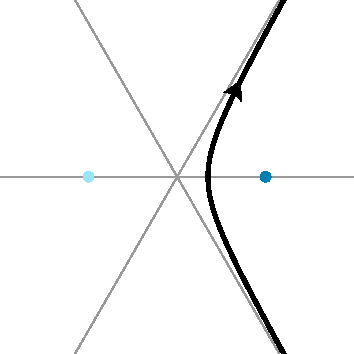
\includegraphics{figures/u_contour_3.pdf} \\[1em]
{\small The contour $\Gamma$ in the $u$ plane.}
\end{center}
With the substitution $t = 2uy^{1/2}$, we can rewrite the Airy integral as
\[ \Ai(y) = y^{1/2}\;\frac{i}{\pi} \int_{y^{-1/2} \Gamma} \exp\left[-\tfrac{2}{3}y^{3/2} \left(4u^3 - 3u\right)\right]\,du. \]
We've rescaled the contour by a factor of two, but it still approaches $\infty$ in the desired way. Note that $4u^3 - 3u$ is the third Chebyshev polynomial.
\subsection{Rewriting as a modified Bessel equation}
We can distill the most interesting part of the Airy function by writing
\[ \Ai(y) = \tfrac{1}{\pi\sqrt{3}}\,y^{1/2}\,K\big(\tfrac{2}{3} y^{3/2}\big), \]
where
\begin{equation}\label{integral:mod-bessel}
K(z) = i\sqrt{3} \int_{z^{-1/3}\Gamma} \exp\left[-z \left(4u^3 - 3u\right)\right]\,du.
\end{equation}
Saying that $\Ai$ satisfies the Airy equation is equivalent to saying that $K$ satisfies the modified Bessel equation
\begin{equation}\label{eqn:mod-bessel}
\left[z^2 \big(\tfrac{\partial}{\partial z}\big)^2 + z \tfrac{\partial}{\partial z} - \big[\big(\tfrac{1}{3}\big)^2 + z^2\big]\right] \varphi = 0.
\end{equation}
In fact, $K$ is the modified Bessel function $K_{1/3}$~\cite[equation~9.6.1]{dlmf}.

The method we'll demonstrate in Section~\ref{spatial} works for any differential equation
\[ \left[ P\big(\tfrac{\partial}{\partial z}\big) + z^{-1} Q\big(\tfrac{\partial}{\partial z}\big) + z^{-2} R(z^{-1}) \right] \varphi = 0, \]
where $P$ is a polynomial, $Q$ is a polynomial of one degree lower, and $R$ is an entire function. Let's put equation~\ref{eqn:mod-bessel} in that form:
\begin{equation}\label{eqn:reg-mod-bessel}
\left[ \big[ \big(\tfrac{\partial}{\partial z}\big)^2 - 1 \big] + z^{-1} \tfrac{\partial}{\partial z} - \big(\tfrac{1}{3}\big)^2 z^{-2} \right] \varphi = 0.
\end{equation}
\subsection{Asymptotic analysis}
Equation~\ref{eqn:mod-bessel} has a regular singularity at $z = 0$ and an irregular singularity at $z = \infty$. From the general theory of such equations, we know that the space of trans-series solutions has a basis of trans-monomials
\[ \{ e^{-\alpha z} z^{-\tau_\alpha}\,\series{W}_\alpha \mid \alpha^2 - 1 = 0 \} \]
where the $\series{W}_\alpha$ are formal power series in $z^{-1}$ with no constant term. From equations 10.40.2 and 10.17.1 of \cite{dlmf}, we learn that $K \sim \left(\tfrac{\pi}{2}\right)^{1/2} e^{-z} z^{1/2}\,\series{W}_1$, with
\begin{equation}\label{bessel-asymp}
\series{W}_1 = z^{-1} - \frac{(\tfrac{1}{6})_1 (\tfrac{5}{6})_1}{2^1 \cdot 1!}\;z^{-2} + \frac{(\tfrac{1}{6})_2 (\tfrac{5}{6})_2}{2^2 \cdot 2!}\;z^{-3} - \frac{(\tfrac{1}{6})_3 (\tfrac{5}{6})_3}{2^3 \cdot 3!}\;z^{-4} + \ldots
\end{equation}

The holomorphic analysis in Section~\ref{spatial} will give us holomorphic solutions
\[ \{ e^{-\alpha z} z^{-\tau_\alpha}\,W_\alpha \mid \alpha^2 - 1 = 0 \}, \]
which seem analogous to the trans-monomials above. Borel summation makes the analogy precise. We'll see in Section~\ref{bessel-regularity} that each $z^{\tau_\alpha}\,W_\alpha$ is proportional to the Borel sum of $z^{\tau_\alpha}\,\series{W}_\alpha$.
\subsection{Going to the spatial domain}\label{spatial}
\subsubsection{The big idea}\label{big-idea}
We're going to look for functions $v_\alpha$ whose Laplace transforms $\laplace_{\zeta, \alpha} v_\alpha$ satisfy equation~\ref{eqn:reg-mod-bessel}. We'll succeed when $\alpha^2 - 1 = 0$, and we'll see that $K$ is a scalar multiple of $\laplace_{\zeta, 1} v_1$.

We can see from Section~\ref{L-int-op} that $\laplace_{\zeta, \alpha} v$ satisfies the differential equation~\ref{eqn:reg-mod-bessel} if and only if $v$ satisfies the integral equation
\begin{equation}\label{int-eq:spatial-mod-bessel}
\left[ \big[ \zeta^2 - 1 \big] - \fracderiv{-1}{\zeta}{\alpha} \circ \zeta - \big(\tfrac{1}{3}\big)^2 \fracderiv{-2}{\zeta}{\alpha} \right] v = 0.
\end{equation}
It's tempting to differentiate both sides of this equation until we get
\begin{equation}\label{diff-eq:spatial-mod-bessel}
\left[ \big(\tfrac{\partial}{\partial \zeta}\big)^2 \circ \big[ \zeta^2 - 1 \big] - \tfrac{\partial}{\partial \zeta} \circ \zeta - \big(\tfrac{1}{3}\big)^2 \right] v = 0,
\end{equation}
which is easier to solve. Unfortunately, a solution of equation~\ref{diff-eq:spatial-mod-bessel} won't satisfy equation~\ref{int-eq:spatial-mod-bessel} in general. However, as we learned in Section~\ref{shifting}, a solution of equation~\ref{diff-eq:spatial-mod-bessel} {\em will} satisfy equation~\ref{int-eq:spatial-mod-bessel} if it's slight and locally integrable at $\zeta = \alpha$.

This is great news, because equation~\ref{diff-eq:spatial-mod-bessel} has a regular singularity at each root of $\zeta^2 - 1$, and the Frobenius method often gives a slight solution at each regular singular point. We can see the regular singularities by moving the derivatives to the right:
\[ \left[ (\zeta^2 - 1) \big(\tfrac{\partial}{\partial \zeta}\big)^2 + 3\zeta \tfrac{\partial}{\partial \zeta} + \big[ 1 - \big(\tfrac{1}{3}\big)^2 \big] \right] v = 0. \]

In Sections \ref{pos-root}\,--\,\ref{neg-root}, we'll see this approach succeed. For each root $\alpha$, we'll find a solution $v_\alpha$ of equation~\ref{diff-eq:spatial-mod-bessel} which is slight and locally integrable at $\zeta = \alpha$. We know the function $\laplace_{\zeta, \alpha} v_\alpha$ will satisfy equation~\ref{eqn:reg-mod-bessel}, and we can even find its asymptotics from the order $\tau_\alpha$ of $v_\alpha$. We learned in Section~\ref{translation} that
\[ \laplace_{\zeta, \alpha} v_\alpha = e^{-\alpha z} V_\alpha \]
where $V_\alpha = \laplace_{\zeta_\alpha, 0} v_\alpha$ and $\zeta = \alpha + \zeta_\alpha$. We can see from Section~\ref{reg-decay} that $V_\alpha$ is asymptotic to a scalar multiple of $z^{-1 - \tau_\alpha}$ at $z = \infty$, so the further decomposition
\[ \laplace_{\zeta, \alpha} v_\alpha = e^{-\alpha z} z^{-\tau_\alpha} W_\alpha, \]
makes $W_\alpha$ is asymptotic to a scalar multiple of $z^{-1}$ at $z = \infty$.
\color{Peru}
\begin{align*}
\left[ \big(\tfrac{\partial}{\partial \zeta}\big)^2 \circ (\zeta - 1)(\zeta + 1) - \tfrac{\partial}{\partial \zeta} \circ \zeta - \big(\tfrac{1}{3}\big)^2 \right] v & = 0
\end{align*}
\color{Sienna}
\begin{align*}
\left[ \big[ 2 + 2(2\zeta) \tfrac{\partial}{\partial \zeta} + (\zeta^2 - 1) \big(\tfrac{\partial}{\partial \zeta}\big)^2 \big] - \big[ 1 + \zeta \tfrac{\partial}{\partial \zeta} \big] - \big(\tfrac{1}{3}\big)^2 \right] v & = 0 \\
\left[ (\zeta^2 - 1) \big(\tfrac{\partial}{\partial \zeta}\big)^2 + 3\zeta \tfrac{\partial}{\partial \zeta} + \big[ 1 - \big(\tfrac{1}{3}\big)^2 \big] \right] v & = 0 \\
\left[ (\zeta - 1)(\zeta + 1) \big(\tfrac{\partial}{\partial \zeta}\big)^2 + 3\zeta \tfrac{\partial}{\partial \zeta} + \big[ 1 - \big(\tfrac{1}{3}\big)^2 \big] \right] v & = 0
\end{align*}
\color{black}
%%In terms of the coordinate $\zeta_\alpha$ with $\zeta = \alpha + \zeta_\alpha$, this equation is written
%%\begin{equation}\label{eqn:centered-mod-bessel}
%%\[ \left[ \big[ \zeta_\alpha (\zeta_\alpha + 2\alpha) + \alpha^2 - 1 \big] + \fracderiv{-1}{\zeta_\alpha}{0} \circ \big[ \zeta_\alpha + \alpha \big] - \big(\tfrac{1}{3}\big)^2 \fracderiv{-2}{\zeta_\alpha}{0} \right] w = 0. \]
%%\end{equation}
\subsubsection{Focus on $\zeta = 1$}\label{pos-root}
Let's find a solution of equation~\ref{diff-eq:spatial-mod-bessel} which is slight and locally integrable at $\zeta = 1$. Define a new coordinate $\zeta_1$ on $\C$ so that $\zeta = 1 + \zeta_1$. In this coordinate, equation~\ref{diff-eq:spatial-mod-bessel} looks like
\begin{equation}%%\label{diff-eq:spatial-mod-bessel-pos}
\left[\zeta_1(2 + \zeta_1) \big(\tfrac{\partial}{\partial \zeta_1}\big)^2 + 3(1 + \zeta_1) \tfrac{\partial}{\partial \zeta_1} + \big[1 - \big(\tfrac{1}{3}\big)^2\big]\right] v = 0.
\end{equation}
With another change of coordinate, given by $\zeta_1 = -2\xi_1$, we can rewrite equation~\ref{diff-eq:spatial-mod-bessel} as the hypergeometric equation
\begin{equation}\label{diff-eq:hypergeom-pos}
\left[\xi_1 (1 - \xi_1) \big(\tfrac{\partial}{\partial \xi_1}\big)^2 + 3(\tfrac{1}{2} - \xi_1) \tfrac{\partial}{\partial \xi_1} - \big[1 - \big(\tfrac{1}{3}\big)^2\big]\right] v = 0.
\end{equation}
Looking through the twenty-four expressions for Kummer's six solutions, we find one \cite[formula~15.10.12]{dlmf} which is manifestly slight and locally integrable at $\xi_1 = 0$:
\begin{alignat*}{2}
v_1 &=\;& \hphantom{-i\sqrt{2}}\,\xi_1^{-1/2} & F\big(\tfrac{1}{6}, \tfrac{5}{6}; \tfrac{1}{2}; \xi_1\big) \\
&=\;& -i\sqrt{2}\,\zeta_1^{-1/2} & F\big(\tfrac{1}{6}, \tfrac{5}{6}; \tfrac{1}{2}; -\tfrac{1}{2}\zeta_1\big)
\end{alignat*}
From the argument in Section~\ref{big-idea}, we know that $\laplace_{\zeta, 1} v_1$ satisfies equation~\ref{eqn:mod-bessel}, and can be written as $e^{-z} V_1$, where $V_1 = \laplace_{\zeta_1, 0} v_1$. Since $v_1$ has order $-1/2$, the decomposition $V_1 = z^{1/2} W_1$ makes $W_1$ asymptotic to a scalar multiple of $z^{-1}$ at $z = \infty$.
\subsubsection{Focus on $\zeta = -1$}\label{neg-root}
Let's find a solution of equation~\ref{diff-eq:spatial-mod-bessel} which is slight and locally integrable at $\zeta = -1$. In the rescaled coordinate from Section~\ref{pos-root}, this is the point $\xi_1 = 1$. Looking again through Kummer's table of solutions, we find another expression \cite[formula~15.10.14]{dlmf} which is manifestly slight and locally integrable at $\xi_1 = 1$:
\begin{alignat*}{2}
v_{-1} &=\;& (1-\xi_1)^{-1/2} & F\big(\tfrac{1}{6}, \tfrac{5}{6}; \tfrac{1}{2}; 1-\xi_1\big) \\
&=\;& \sqrt{2}\,\zeta_{-1}^{-1/2} & F\big(\tfrac{1}{6}, \tfrac{5}{6}; \tfrac{1}{2}; \tfrac{1}{2}\zeta_{-1}\big)
\end{alignat*}
where $\zeta_{-1}$ is the coordinate with $\zeta = -1 + \zeta_{-1}$. From the argument in Section~\ref{big-idea}, we know that $\laplace_{\zeta, -1} v_{-1}$ satisfies equation~\ref{eqn:mod-bessel}, and can be written as $e^z V_{-1}$, where $V_{-1} = \laplace_{\zeta_{-1}, 0} v_{-1}$. Since $v_{-1}$, like our other solution, has order $-1/2$, the same decomposition $V_{-1} = z^{1/2} W_{-1}$ makes $W_{-1}$ asymptotic to a scalar multiple of $z^{-1}$ at $z = \infty$.

In this example, $v_1$ and $v_{-1}$ happen to be related by a symmetry: the M\"{o}bius transformation that pulls $\zeta$ back to $-\zeta$. Kummer's solutions typically come from six different hypergeometric equations, which are related by the M\"{o}bius transformations that permute their singularities. In our case, though, exchanging $1$ with $-1$ keeps equation~\ref{diff-eq:spatial-mod-bessel} the same.

\color{DodgerBlue}
If we'd followed the routine from Section~\ref{pos-root}, rewriting equation~\ref{diff-eq:spatial-mod-bessel} in the coordinate $\zeta_{-1}$ and then rewriting it again in a more recognizable form, we would've arrived at the hypergeometric equation
\[ \left[\xi_{-1} (1 - \xi_{-1}) \big(\tfrac{\partial}{\partial \xi_{-1}}\big)^2 + 3(\tfrac{1}{2} - \xi_{-1}) \tfrac{\partial}{\partial \xi_{-1}} - \big[1 - \big(\tfrac{1}{3}\big)^2\big]\right] v = 0, \]
where $\zeta_{-1} = 2\xi_{-1}$. This is the same as what we'd get by substituting $\xi_{-1}$ for $\xi_1$ in Section~\ref{pos-root}! In other words, the holomorphic map that pulls $\xi_{-1}$ back to $\xi_1$
\color{black}
\section{The Airy-Lucas equation}
\subsection{Basics}
The Airy-Lucas equation is
\begin{equation}\label{eqn:airy-lucas}
\left[\big(\tfrac{\partial}{\partial y}\big)^2 - (m-1) y^{-1} \tfrac{\partial}{\partial y} - y^{n-2}\right] \psi = 0
\end{equation}
with $n \in \{3, 4, 5, \ldots\}$ and $m \in \{1, 2, \ldots, r-1\}$. A few solutions are given by the Airy-Lucas functions~\textcolor{magenta}{[Charbonnier et al., equation~3.6]}
\[ \widehat{\Ai}^{(k)}_{n, m-1}(y) = \left\{\begin{array}{ll}1 & j \text{ even} \\ i & j \text{ odd}\end{array}\right\} \frac{y^{m/2}}{\pi} \int_{\Lambda^{(j)}} \exp\left[\tfrac{2}{n} y^{n/2}\,T_n(u)\right]\,U_{m-1}(u)\,du, \]
where $\Lambda^{(k)}$ is the Lefschetz thimble through $u = \cos\big(\tfrac{k}{n}\pi\big)$.
\subsection{Rewriting as a \textcolor{DarkCyan}{modified Bessel (?)} equation}
We can distill the most interesting parts of the Airy-Lucas function by writing
\[ \widehat{\Ai}^{(k)}_{n, m-1}(y) = \textcolor{magenta}{\text{const.}}\,y^{\textcolor{DarkCyan}{m/2}}\,K\big(\tfrac{2}{n} y^{n/2}\big), \]
where
\begin{equation}\label{integral:mod-bessel-rational}
K(z) = \textcolor{magenta}{\text{const.}} \int_{z^{-\textcolor{DarkCyan}{1/n}}\Lambda^{(k)}} \exp\left[-z T_n(u)\right]\,U_{m-1}(u)\,du.
\end{equation}
Saying that $\widehat{\Ai}^{(k)}_{n, m-1}$ satisfies the Airy-Lucas equation is equivalent to saying that $K$ satisfies the \textcolor{DarkCyan}{modified Bessel (?)} equation
\begin{equation}%%\label{eqn:mod-bessel}
\left[z^2 \big(\tfrac{\partial}{\partial z}\big)^2 + z \tfrac{\partial}{\partial z} - \big[\big(\textcolor{DarkCyan}{\tfrac{m}{n} (?)}\big)^2 + z^2\big]\right] \varphi = 0.
\end{equation}
In fact, as we'll see in Section~\textcolor{magenta}{?}, $K$ is the modified Bessel function $K_{\textcolor{DarkCyan}{m/n}}$.

Like we did in equation~\ref{eqn:reg-mod-bessel}, we can rewrite the modified Bessel equation above as
\begin{equation}%%\label{eqn:reg-mod-bessel}
\left[ \big[ \big(\tfrac{\partial}{\partial z}\big)^2 - 1 \big] + z^{-1} \tfrac{\partial}{\partial z} - \big(\textcolor{DarkCyan}{\tfrac{m}{n}}\big)^2 z^{-2} \right] \varphi = 0.
\end{equation}
\section{The higher Airy equation}
\subsection{Basics}
The higher Airy equation is
\begin{equation}\label{eqn:airy-lucas}
\left[\big({-}\tfrac{\partial}{\partial y}\big)^{n-1} - y\right] \psi = 0
\end{equation}
with $n \in \{3, 4, 5, \ldots\}$. A few solutions are given by the hyper-Airy functions~\textcolor{magenta}{[Charbonnier et al., equation~3.6]}

\color{Peru}
With
\begin{align*}
z & = (-1)^{n-1} \tfrac{n-1}{n} y^{n/(n-1)} & w & = (-1)^n (n-1) y^{1/(n-1)} u,
\end{align*}
we have
\begin{align*}
\widetilde{\Ai}^{(k)}_n(y) & = \frac{\exp\big(\pi ik \tfrac{n-2}{n-1}\big)}{2\pi i} \int_{\Lambda^{(j)}} \exp\left[\tfrac{1}{n}w^n - yw\right]\,dw \\
& = \frac{\exp\big(\pi ik \tfrac{n-2}{n-1}\big)}{2\pi i} \int_{\Lambda^{(j)}} \exp\left[\tfrac{1}{n}w \left(w^{n-1} - ny\right)\right]\,dw \\
& = \frac{\exp\big(\pi ik \tfrac{n-2}{n-1}\big)}{2\pi i} \int_{\Lambda^{(j)}} \exp\left[\tfrac{1}{n}w \big((n-1)^{n-1} yu^{n-1} - ny\big)\right]\,dw \\
& = \frac{\exp\big(\pi ik \tfrac{n-2}{n-1}\big)}{2\pi i} \int_{\Lambda^{(j)}} \exp\left[\tfrac{1}{n}yw \big((n-1)^{n-1} u^{n-1} - n\big)\right]\,dw \\
& = \frac{\exp\big(\pi ik \tfrac{n-2}{n-1}\big)}{2\pi i} \int_{\Lambda^{(j)}} \exp\left[(-1)^n \tfrac{n-1}{n} y^{n/(n-1)} u\big((n-1)^{n-1} u^{n-1} - n\big)\right]\,dw \\
& = \frac{\exp\big(\pi ik \tfrac{n-2}{n-1}\big)}{2\pi i} \int_{\Lambda^{(j)}} \exp\left[-z\big((n-1)^{n-1} u^n - nu\big)\right]\,dw \\
& = (-1)^n (n-1) \frac{\exp\big(\pi ik \tfrac{n-2}{n-1}\big)}{2\pi i} y^{1/(n-1)}\int_{\Lambda^{(j)}} \exp\left[-z\big((n-1)^{n-1} u^n - nu\big)\right]\,du \\
& = (-1)^n (n-1) \frac{\exp\left(\pi ik \big(1 - \tfrac{1}{n-1}\big)\right)}{2\pi i} y^{1/(n-1)}\int_{\Lambda^{(j)}} \exp\left[-z\big((n-1)^{n-1} u^n - nu\big)\right]\,du \\
& = (-1)^{n+k} (n-1) \frac{\exp\big({-}\pi i \tfrac{k}{n-1}\big)}{2\pi i} y^{1/(n-1)}\int_{\Lambda^{(j)}} \exp\left[-z\big((n-1)^{n-1} u^n - nu\big)\right]\,du \\
\end{align*}
\color{black}
\[ \widetilde{\Ai}^{(k)}_n(y) = (-1)^{n+k} (n-1) \frac{\exp\big({-}\pi i \tfrac{k}{n-1}\big)}{2\pi i} y^{1/(n-1)}\int_{\Lambda^{(j)}} \exp\left[-z\big((n-1)^{n-1} u^n - nu\big)\right]\,du \\, \]
where $\Lambda^{(k)}$ is the Lefschetz thimble through $u = \cos\big(\tfrac{k}{n}\pi\big)$.
\subsection{Rewriting as a \textcolor{magenta}{(???)} equation}
We can distill the most interesting parts of the hyper-Airy function by writing
\[ \widetilde{\Ai}^{(k)}_n(y) = \textcolor{magenta}{\text{const.}}\,y^{1/(n-1)}\,K\left((-1)^n\,\tfrac{n-1}{n}\,y^{n/(n-1)}\right), \]
where
\begin{equation}
K(z) = \textcolor{magenta}{\text{const.}} \int_{\textcolor{magenta}{\text{const.}(n)} z^{-\textcolor{DarkCyan}{1/n}}\Lambda^{(k)}} \exp\left[-z\big((n-1)^{n-1} u^n - nu\big)\right]\,du.
\end{equation}
Saying that $\widetilde{\Ai}^{(k)}_n$ satisfies the higher Airy equation is equivalent to saying that $K$ satisfies an equation of the form
\begin{equation}%%\label{eqn:mod-bessel}
\left[ \big[ \big({-}\tfrac{\partial}{\partial z}\big)^{n-1} - 1 \big] - c_n^{(1)} z^{-1} \big({-}\tfrac{\partial}{\partial z}\big)^{n-2} - c_n^{(2)} z^{-2} \big({-}\tfrac{\partial}{\partial z}\big)^{n-3} - \ldots - c_n^{(n-1)} z^{-(n-1)} \right] \varphi = 0.
\end{equation}
The sub-leading coefficients are the triangular numbers
\[ c_n^{(1)} = \frac{n(n-1)}{2}. \]
\color{DarkCyan}
The later coefficients can be written as\footnote{Many thanks to Peter Taylor for noticing this [\url{https://mathoverflow.net/q/422337/1096}].}
\[ c_n^{(k)} = \frac{b_n^{(k)}}{n^k}\,(n+1)^{\underline{k+2}} \]
in terms of the polynomials
\begin{equationarray*}{*{11}{c}}
b_n^{(2)} & = & \tfrac{1}{24} \\
b_n^{(3)} & = & \tfrac{1}{48} n \\
b_n^{(4)} & = & \tfrac{73}{5760} n^2 & + & \tfrac{1}{1152} n & - & \tfrac{1}{2880} \\
b_n^{(5)} & = & \tfrac{11}{1280} n^{3} & + & \tfrac{1}{768} n^{2} & - & \tfrac{1}{1920} n \\
b_n^{(6)} & = & \tfrac{3625}{580608} n^{4} & + & \tfrac{61}{41472} n^{3} & - & \tfrac{181}{322560} n^{2} & - & \tfrac{1}{41472} n & + & \tfrac{1}{181440}. \end{equationarray*}
Searching for 580608 in the OEIS turns up the leading coefficients $\beta^{(k)}$ of these polynomials, which are listed as {\tt A249276} and {\tt A249277}. They're defined by the identity [Yang, ``Approximations for Constant $e$ and Their Applications'']
\[ \frac{1}{e} \left(\frac{n}{n-1}\right)^{n-1} = 1 - \frac{1/2}{n} - \frac{\beta^{(2)}}{n^2} - \frac{\beta^{(3)}}{n^3} - \frac{\beta^{(4)}}{n^4} - \frac{\beta^{(5)}}{n^5} - \ldots, \]
which tells us that
\[ \frac{1}{e} \left(\frac{n}{n-1}\right)^{n-1} = 1 - \frac{1/2}{n} - \frac{b_n^{(2)}}{n^2} - \frac{b_n^{(3)}}{n^4} - \left[\frac{b_n^{(4)}}{n^6} + o\left(\frac{1}{n^5}\right)\right] - \left[\frac{b_n^{(5)}}{n^8} + o\left(\frac{1}{n^6}\right)\right] - \ldots. \]
The last coefficient can be written as
\[ c_n^{(n-1)} = \left(\frac{n-1}{n}\right)^{n-1} \left(\frac{1}{n-1}\right)^{\underline{n-1}}, \]
giving
\[ b_n^{(n-1)} = (n-1)^{n-1} \left(\frac{1}{n-1}\right)^{\underline{n-1}} \Big/ (n+1)^{\underline{n+1}}. \]
\color{black}
\section{Sketches}
\subsection{Contour argument for the Airy function}\label{contour-argument}
We can recast integral~\ref{integral:mod-bessel} into the $\zeta$ plane by setting $\zeta = 4u^3 - 3u$. Projecting $z^{-1/3} \Gamma$ to a contour $\gamma_z$ in the $\zeta$ plane and choosing the branch of $u$ that lifts $\gamma_z$ back to $z^{-1/3} \Gamma$, we have
\begin{equation}\label{integral:mod-bessel-zeta}
K = \frac{i}{\sqrt{3}} \int_{\gamma_z} e^{-z\zeta}\frac{d\zeta}{4u^2 - 1}.
\end{equation}
For $z \in (0, \infty)$, the contour $\gamma_z$ runs clockwise around $[1, \infty)$, as shown below. Let's assume $z \in (0, \infty)$ for the rest of the section. \textcolor{magenta}{[Our conclusions should probably hold whenever $\operatorname{Re}(z) > 0$.]}
\begin{center}
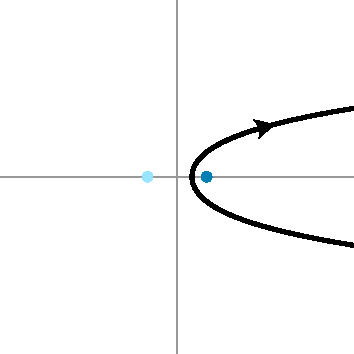
\includegraphics{figures/zeta_contour_3.pdf} \\[1em]
{\small The contour $\gamma_1$ in the $\zeta$ plane.}
\end{center}

It happens\footnote{\textcolor{magenta}{Veronica:} This comes from \cite[equation~15.4.14]{dlmf}.} that for our desired branch of $u$,
\[ \frac{1}{4u^2 - 1} = -F\big(\tfrac{1}{3}, \tfrac{2}{3}; \tfrac{1}{2}; \zeta^2\big), \]
so we can rewrite integral~\ref{integral:mod-bessel-zeta} as
\[ K = \frac{1}{i\sqrt{3}} \int_{\gamma_z} e^{-z\zeta} F\big(\tfrac{1}{3}, \tfrac{2}{3}; \tfrac{1}{2}; \zeta^2\big)\;d\zeta. \]
This gives us an alternate route to the conclusion of Section~\ref{spatial}, which we'll follow below.

In addition to the solutions $g_1$ and $f_0$ from Section~\ref{spatial-success}, equation~\ref{eqn:hypergeom} has the solutions
\begin{alignat*}{2}
g_0 &\;=\;& & F\big(\tfrac{2}{3}, \tfrac{4}{3}; \tfrac{3}{2}; 1-\xi\big) \\
f_1 &\;=\;& (1-\xi)^{-1/2} & F\big(\tfrac{1}{6}, \tfrac{5}{6}; \tfrac{1}{2}; 1-\xi\big),
\end{alignat*}
given by formulas 15.10.13 and 15.10.14 from \cite{dlmf}.

The quadratic transformation identity 15.8.27 from \cite{dlmf} shows \textcolor{magenta}{[verified numerically]} that\footnote{Note that $2\Gamma(\tfrac{1}{2})\Gamma(\tfrac{3}{2}) = 2\Gamma(\tfrac{1}{2})\,\tfrac{1}{2}\Gamma(\tfrac{1}{2}) = \pi$ and $\big[\Gamma(\tfrac{5}{6})\Gamma(\tfrac{7}{6})\big]^{-1} = \big[\Gamma(\tfrac{5}{6})\,\tfrac{1}{6}\Gamma(\tfrac{1}{6})\big]^{-1} = \frac{6\sin(\tfrac{1}{6} \pi)}{\pi} = \frac{3}{\pi}$.}
\[ F\big(\tfrac{1}{3}, \tfrac{2}{3}; \tfrac{1}{2}; \zeta^2\big) = \tfrac{1}{3}(g_1 + g_0), \]
so we have
\[ K = \frac{1}{i\,3\sqrt{3}} \int_{\gamma_z} e^{-z\zeta} (g_1 + g_0)\;d\zeta. \]
The solution $g_1$ is holomorphic on $\zeta \in [1, \infty)$, so it integrates to zero. The solution $g_0$, in contrast, is non-meromorphic at $\zeta = 1$. Along the branch cut $\zeta \in [1, \infty)$, its above-minus-below difference is $-\tfrac{3\sqrt{3}}{2}\,f_0$,
as given\footnote{Note that $\Gamma(\tfrac{3}{2}) \Gamma(\tfrac{1}{2})^{-1} = \tfrac{1}{2}$ and $\big[\Gamma(\tfrac{2}{3})\Gamma(\tfrac{4}{3})\big]^{-1} = \big[\Gamma(\tfrac{2}{3})\,\tfrac{1}{3}\Gamma(\tfrac{1}{3})\big]^{-1} = \frac{3\sin(\tfrac{1}{3} \pi)}{\pi} = \frac{3\sqrt{3}}{2\pi}$.} by equation~15.2.3 from \cite{dlmf}.
Hence,
\begin{align*}
K & = \frac{i}{2} \int^\infty_1 e^{-z\zeta} f_0\;d\zeta \\
e^z K & = \frac{i}{2} \int^\infty_1 e^{-z(\zeta - 1)} f_0\;d\zeta \\
K_1 & = \tfrac{i}{2} \laplace_{\zeta_1} f_0,
\end{align*}
just as we found in Section~\ref{spatial-success}.
\subsection{Another solution}
Section~\ref{contour-argument} associates the solution $K$ of equation~\ref{eqn:mod-bessel} with the solution $g_0$ of equation~\ref{eqn:hypergeom}, which contributes the pole at $\zeta = 1$ of
\[ \frac{du}{d\zeta} = \frac{1}{4u^2 - 1} = \tfrac{1}{3}(g_1 + g_0). \]
The solution $g_1$, which contributes the pole at $\zeta = -1$, is associated with another solution of equation~\ref{eqn:mod-bessel}.

To express this other solution as a Laplace transform, following the method of Section~\ref{spatial-success}, we would use the solution
\[ f_1 = (1-\xi)^{-1/2} F\big(\tfrac{1}{6}, \tfrac{5}{6}; \tfrac{1}{2}; 1-\xi\big) \]
of equation~\ref{eqn:hypergeom}, given by formula~15.10.14 from \cite{dlmf}. This is the only solution, up to scale, which has a fractional power singularity at $\zeta = -1$.

In summary, the contour integration method of solving equation~\ref{eqn:mod-bessel} is associated with the basis
\begin{align*}
g_1 & = F\big(\tfrac{2}{3}, \tfrac{4}{3}; \tfrac{3}{2}; \xi\big) \\
g_0 & = F\big(\tfrac{2}{3}, \tfrac{4}{3}; \tfrac{3}{2}; 1-\xi\big)
\end{align*}
of solutions for equation~\ref{eqn:hypergeom}, given by formulas 15.10.11 and 15.10.13 from \cite{dlmf}. These solutions contribute the poles at $\xi = 1$ and $\xi = 0$, respectively, of a generic solution.

The Laplace transformation method of solving equation~\ref{eqn:mod-bessel}, on the other hand, is associated with the basis
\begin{alignat*}{2}
f_1 &\;=\;& (1-\xi)^{-1/2} & F\big(\tfrac{1}{6}, \tfrac{5}{6}; \tfrac{1}{2}; 1-\xi\big) \\
f_0 &\;=\:& \xi^{-1/2} & F\big(\tfrac{1}{6}, \tfrac{5}{6}; \tfrac{1}{2}; \xi\big)
\end{alignat*}
given by formulas 15.10.14 and 15.10.12 from \cite{dlmf}. These solutions, up to scale, are the only ones with fractional power singularities.

Identities 15.10.18, and 15.10.22 from \cite{dlmf} give the change of basis
\begin{alignat*}{3}
f_1 &\;=\;&\tfrac{1}{\sqrt{3}}\,g_1 &\;+\;& \tfrac{1}{2}\,f_0 \\
f_0 &\;=\;& \tfrac{1}{\sqrt{3}}\,g_0 &\;+\;& \tfrac{1}{2}\,f_1.
\end{alignat*}
Summing these identities, we see that
\[ g_1 + g_0 = \tfrac{\sqrt{3}}{2}\,(f_1 + f_0), \]
giving the alternate decomposition
\[ \frac{du}{d\zeta} = \tfrac{1}{2\sqrt{3}}\,(f_1 + f_0). \]
\subsection{Contour argument for Airy-Lucas functions}
Generalizing from Section~\ref{contour-argument}, we can recast integral~\ref{integral:mod-bessel-rational} into the $\zeta$ plane by setting $\textcolor{magenta}{-\zeta} = T_n(u)$, which implies that $-d\zeta = n U_{n-1}(u)\,du$. Projecting as before, we get \textcolor{magenta}{[sign flipped]} \textcolor{DarkCyan}{[see identity in \texttt{cyl-resurgence.tex}]}
\begin{align*}%%\label{integral:mod-bessel-rational-zeta}
K_{m/n}(z) & = \frac{n}{2 \sinh\big(\tfrac{m}{n}\,i\pi\big)} \int_{z^{-\textcolor{DarkCyan}{1/n}}\Lambda^{(k)}} \exp\left[z T_n(u)\right]\,U_{m-1}(u)\,du \\
& = -\frac{1}{2 \sinh\big(\tfrac{m}{n}\,i\pi\big)} \int_{\gamma_z} e^{-z\zeta}\,\frac{U_{m-1}(u)}{U_{n-1}(u)}\,d\zeta \\
& = -\frac{1}{2\,\tfrac{n}{m} \sinh\big(\tfrac{m}{n}\,i\pi\big)} \int_{\gamma_z} e^{-z\zeta}\,F(1 - \tfrac{m}{n}, 1 + \tfrac{m}{n}, \tfrac{3}{2}, \tfrac{1}{2} \pm \tfrac{1}{2}\zeta)\,d\zeta.
\end{align*}
\textcolor{DarkCyan}{where the sign must be chosen so that $\pm\zeta$ stays in the left half-plane over the whole integration path (?)}.
For $z \in (0, \infty)$, the contour $\gamma_z$ runs \textcolor{magenta}{counterclockwise} around $[1, \infty)$, as shown below\textcolor{DarkCyan}{, so we have to choose the negative sign above (?)}. Let's assume $z \in (0, \infty)$ for the rest of the section. \textcolor{magenta}{[Our conclusions should probably hold whenever $\operatorname{Re}(z) > 0$.]}
\begin{center}
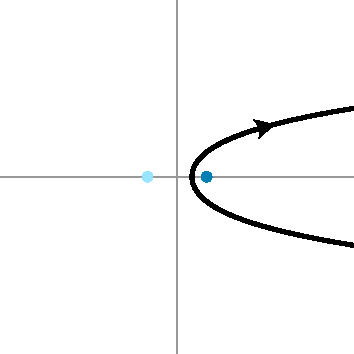
\includegraphics{figures/zeta_contour_3.pdf} \\[1em]
{\small The contour $\gamma_1$ \textcolor{magenta}{[reversed]} in the $\zeta$ plane.}
\end{center}

The integrand is non-meromorphic at $\zeta = 1$. Along the branch cut $\zeta \in [1, \infty)$, its above-minus-below difference is
\begin{align*}
& -(2\pi i)\tfrac{n}{2\pi m} \sin(\tfrac{m}{n} \pi)\,(\pm\tfrac{1}{2}\zeta - \tfrac{1}{2})^{-1/2} F(\tfrac{1}{2} + \tfrac{m}{n}, \tfrac{1}{2} - \tfrac{m}{n}, \tfrac{1}{2}, \tfrac{1}{2} \mp \tfrac{1}{2}\zeta) \\
= & -\tfrac{n}{m} \sinh(\tfrac{m}{n}\,i\pi)\,(\pm\tfrac{1}{2}\zeta - \tfrac{1}{2})^{-1/2} F(\tfrac{1}{2} + \tfrac{m}{n}, \tfrac{1}{2} - \tfrac{m}{n}, \tfrac{1}{2}, \tfrac{1}{2} \mp \tfrac{1}{2}\zeta),
\end{align*}
as given\footnote{Note that $\Gamma(\tfrac{3}{2}) \Gamma(\tfrac{1}{2})^{-1} = \tfrac{1}{2}$ and $\big[\Gamma(1 - \tfrac{m}{n})\Gamma(1 + \tfrac{m}{n})\big]^{-1} = \big[\Gamma(1 - \tfrac{m}{n})\,\tfrac{m}{n}\Gamma(\tfrac{m}{n})\big]^{-1} = \tfrac{n}{m\pi} \sin(\tfrac{m}{n} \pi)$.} by equation~15.2.3 from \cite{dlmf}. Hence, $K_{m/n}$ turns out to be the Laplace transform along $(1, \infty)$ of
\[ \tfrac{1}{2}\,(-\tfrac{1}{2}\zeta - \tfrac{1}{2})^{-1/2} F(\tfrac{1}{2} + \tfrac{m}{n}, \tfrac{1}{2} - \tfrac{m}{n}, \tfrac{1}{2}, \tfrac{1}{2} + \tfrac{1}{2}\zeta). \]
\color{DarkCyan}
Guessing the branch of the square root for consistency with the numerically checked result in Section~\ref{contour-argument}, we get
\[ \tfrac{i}{2}\,(\tfrac{1}{2} + \tfrac{1}{2}\zeta)^{-1/2} F(\tfrac{1}{2} + \tfrac{m}{n}, \tfrac{1}{2} - \tfrac{m}{n}, \tfrac{1}{2}, \tfrac{1}{2} + \tfrac{1}{2}\zeta). \]
In other words, $K_{m/n} = \tfrac{i}{2} \laplace_{\zeta, -1} v_{-1}$ with
\[ v_{-1} = \sqrt{2}\,\zeta_{-1}^{-1/2} F(\tfrac{1}{2} + \tfrac{m}{n}, \tfrac{1}{2} - \tfrac{m}{n}, \tfrac{1}{2}, \tfrac{1}{2}\zeta_{-1}), \]
where $\zeta = -1 + \zeta_{-1}$.
\color{black}
\subsection{Lifting to a countable cover}
Formula~\ref{integral:mod-bessel-rational} expresses the modified Bessel function $K_{m/n}$ as an exponential integral on a finite cover of $\C$. Lifting to a countable cover reveals this formula as a special case of a general integral formula for modified Bessel functions.

Setting $u = \cosh(t/n)$ and recalling that
\begin{align*}
\cosh(n\tau) & := T_n(\cosh(\tau)) \\
\sinh(m\tau) & := U_{m-1}(\cosh(\tau)) \sinh(\tau),
\end{align*}
we can rewrite formula~\ref{integral:mod-bessel-rational} as \textcolor{magenta}{[switching to the conventional sign for the projection map, so $\Lambda^{(3)}$ now comes from $\infty$ at $-60^\circ$ and goes to $\infty$ at $60^\circ$]}
\begin{align}
\notag K_{m/n}(z) & = \frac{n}{2 \sinh\big(\tfrac{m}{n}\,i\pi\big)} \int_{z^{-\textcolor{DarkCyan}{1/n}}\Lambda^{(k)}} \exp\left[z T_n(u)\right]\,U_{m-1}(u)\,du \\
\notag & = \frac{n}{2 \sinh\big(\tfrac{m}{n}\,i\pi\big)} \int_{\textcolor{magenta}{\Omega}} \exp\left[z \cosh(t)\right]\,U_{m-1}(\cosh(t/n))\,\sinh(t/n)\,d(t/n) \\
\label{integral:mod-bessel-lifted} & = \frac{1}{2 \sinh\big(\tfrac{m}{n}\,i\pi\big)} \int_{\textcolor{magenta}{\Omega}} \exp\left[z \cosh(t)\right]\,\sinh\big(\tfrac{m}{n}\,t\big)\,dt.
\end{align}
For any $\nu \in \C \smallsetminus \Z$, formulas~10.27.4 and 10.32.12 from \cite{dlmf} tell us that
\begin{align}
\notag K_\nu(z) & = \frac{\pi}{\sin(\nu \pi)} \cdot \frac{1}{2}\big[ I_{-\nu}(z) - I_\nu(z) \big] \\
\notag & = \frac{1}{2i \sin(\nu \pi)} \int_\Omega \exp\left[z \cosh(t)\right]\,\frac{1}{2}\left[e^{\nu t} - e^{-\nu t}\right]\,dt \\
\label{intgral:mod-bessel-general} & = \frac{1}{2 \sinh(\nu\,i\pi)} \int_\Omega \exp\left[z \cosh(t)\right]\,\sinh(\nu t)\,dt,
\end{align}
where $\Omega$ is a path that comes from $\infty$ along $-i \pi + (0, \infty)$ and goes to $\infty$ along $i \pi + (0, \infty)$. The integral converges when $z$ is in the right half-plane. We get formula~\ref{integral:mod-bessel-lifted} when we choose a rational parameter $\nu = m/n$.

When $\nu$ goes to $0$, formula~\ref{integral:mod-bessel-lifted} becomes
\[ K_\nu(z) = \frac{1}{2\pi i} \int_\Omega \exp\left[z \cosh(t)\right]\,t\,dt. \]
Choosing $\Omega$ to be the unit-speed path that runs from $\infty$ leftward to $-i\pi$, upward to $i\pi$, and rightward back to $\infty$, we can rewrite this formula as
\begin{align*}
K_\nu(z) & = \frac{1}{2\pi i} \int_0^\infty \exp\left[-z \cosh(t)\right]\,2\pi i\,dt \\
& = \int_0^\infty \exp\left[-z \cosh(t)\right]\,dt \\
& = \int_1^\infty \exp\left[-z\,\tfrac{1}{2}\left(s + \tfrac{1}{s}\right)\right]\,\frac{ds}{s},
\end{align*}
with $s = e^t$. This is a special case of formula~10.32.9 from \cite{dlmf}.
\subsection{Link to dihedral triangulations}
Here are the local normal forms of Kummer's first and second solutions. In the table, $[\bullet]$ denotes a local holomorphic function of order $0$ \cite[identities 15.8.2--4]{dlmf}, and
\begin{align*}
a' & = a+(1-c) \\
b' & = b+(1-c) \\
c' & = 2-c
\end{align*}
\begin{center}
\begin{tabular}{c|c|c|c}
Function & $0$ & $1$ & $\infty$ \\ \hline
$F(a, b, c, \xi)$ & $[\bullet]$ & $[\bullet] + (1-\xi)^{c-a-b} [\bullet]$ & $(1/\xi)^a [\bullet] + (1/\xi)^b [\bullet]$ \\
$\xi^{1-c} F(a', b', c', \xi)$ & $\xi^{1-c} [\bullet]$ & $[\bullet] + (1-\xi)^{c-a-b} [\bullet]$ & $(1/\xi)^a [\bullet] + (1/\xi)^b [\bullet]$
\end{tabular}
\end{center}

For example, at $\zeta = \infty$, the function
\[ u_{-1} = F(1 - \tfrac{m}{n}, 1 + \tfrac{m}{n}, \tfrac{3}{2}, 1 - \tfrac{1}{2} \zeta_{-1}) \]
is slight, with normal form $(1/\zeta_{-1})^{1 - m/n} f_1 + (1/\zeta_{-1})^{1 + m/n} f_2$~\cite[identity~15.8.3]{dlmf}. At $\zeta = 1$, it's holomorphic with order $0$. At $\zeta = -1$, it has the form $h + \zeta_{-1}^{-1/2} f$, where $h$ is holomorphic with order $0$.

On the other hand, the function
\[ v_{-1} = \sqrt{2}\,\zeta_{-1}^{-1/2} F(\tfrac{1}{2} + \tfrac{m}{n}, \tfrac{1}{2} - \tfrac{m}{n}, \tfrac{1}{2}, \tfrac{1}{2}\zeta_{-1}) \]
is slight at $\zeta = \pm 1$ with order $-\tfrac{1}{2}$, and slight at $\infty$ with order $1 - \tfrac{m}{n}$.

Hence, the ratio $u_{-1} / v_{-1}$ looks like a holomorphic multiple of $\zeta_1^{1/2}$ near $\zeta = 1$, a holomorphic function plus a holomorphic multiple of $\zeta_{-1}^{1/2}$ near $\zeta = -1$, and a holomorphic function plus a holomorphic multiple of $(1/\zeta_{-1})^{2m/n}$ near $\zeta = \infty$. This is consistent with $u_{-1}/v_{-1}$ being a conformal map that sends the upper half-plane to a triangle with interior angle $\pi/2$ at the images of $\zeta = \pm 1$ and interior angle $2\pi\,\tfrac{m}{n}$ at the image of $\infty$.

\color{ForestGreen}
Let's try to get the small tetrahedral tiling by setting
\begin{align*}
1 - c & = \tfrac{1}{3} \\
c - a - b & = \tfrac{1}{3} \\
b - a & = \tfrac{1}{2},
\end{align*}
so $(a, b, c) = (-\tfrac{1}{12}, \tfrac{5}{12}, \tfrac{2}{3})$. The general hypergeometric equation is
\begin{align*}
\left[\xi_1 (1 - \xi_1) \big(\tfrac{\partial}{\partial \xi_1}\big)^2 + \big[c - (a+b+1)\xi_1\big] \tfrac{\partial}{\partial \xi_1} - ab\right] & v = 0 \\
\left[-\tfrac{1}{2}\zeta_1 (1 + \tfrac{1}{2}\zeta_1) 4 \big(\tfrac{\partial}{\partial \zeta_1}\big)^2 + \big[c + \tfrac{1}{2}(a+b+1)\zeta_1\big] (-2) \tfrac{\partial}{\partial \zeta_1} - ab\right] & v = 0 \\
\left[-\zeta_1 (2 + \zeta_1) \big(\tfrac{\partial}{\partial \zeta_1}\big)^2 - \big[2c + (a+b+1)\zeta_1\big] \tfrac{\partial}{\partial \zeta_1} - ab\right] & v = 0 \\
\left[(1 - \zeta)(1 + \zeta) \big(\tfrac{\partial}{\partial \zeta}\big)^2 - \big[2c + (a+b+1)(\zeta - 1)\big] \tfrac{\partial}{\partial \zeta} - ab\right] & v = 0 \\
\left[(1 - \zeta^2)\big(\tfrac{\partial}{\partial \zeta}\big)^2 - \big[(c - a - b) + (c - 1) + (a+b+1)\zeta\big] \tfrac{\partial}{\partial \zeta} - ab\right] & v = 0 \\
\left[(1 - \zeta^2)\big(\tfrac{\partial}{\partial \zeta}\big)^2 - \big[\mu - \lambda + (a+b+1)\zeta\big] \tfrac{\partial}{\partial \zeta} - ab\right] & v = 0 \\
\left[\big[\tfrac{\partial}{\partial \zeta} \circ (1 - \zeta^2) + 2\zeta\big] \tfrac{\partial}{\partial \zeta} - (\mu - \lambda) \tfrac{\partial}{\partial \zeta} - (a+b+1)\big[\tfrac{\partial}{\partial \zeta} \circ \zeta - 1\big] - ab\right] & v = 0 \\
\left[\tfrac{\partial}{\partial \zeta} \circ \big[ \tfrac{\partial}{\partial \zeta} \circ (1 - \zeta^2) + 2\zeta \big] + 2\big[\tfrac{\partial}{\partial \zeta} \circ \zeta - 1\big] - (\mu - \lambda) \tfrac{\partial}{\partial \zeta} - (a+b+1)\big[\tfrac{\partial}{\partial \zeta} \circ \zeta - 1\big] - ab\right] & v = 0 \\
\left[\big[ \big(\tfrac{\partial}{\partial \zeta}\big)^2 \circ (1 - \zeta^2) + 4 \tfrac{\partial}{\partial \zeta} \circ \zeta - 2 \big] - (\mu - \lambda) \tfrac{\partial}{\partial \zeta} - (a+b+1) \tfrac{\partial}{\partial \zeta} \circ \zeta + \big[ (a+b+1) - ab \big]\right] & v = 0 \\
\left[\big(\tfrac{\partial}{\partial \zeta}\big)^2 \circ (1 - \zeta^2) - (\mu - \lambda) \tfrac{\partial}{\partial \zeta} + (3-a-b) \tfrac{\partial}{\partial \zeta} \circ \zeta + \big[ {-}1 + a + b - ab \big]\right] & v = 0 \\
\left[\big(\tfrac{\partial}{\partial \zeta}\big)^2 \circ (1 - \zeta^2) - (\mu - \lambda) \tfrac{\partial}{\partial \zeta} + (3-a-b) \tfrac{\partial}{\partial \zeta} \circ \zeta - (a-1)(b-1)\right] & v = 0 \\
\left[\big(\tfrac{\partial}{\partial \zeta}\big)^2 \circ (\zeta^2 - 1) + (\mu - \lambda) \tfrac{\partial}{\partial \zeta} + (a+b-3) \tfrac{\partial}{\partial \zeta} \circ \zeta + (a-1)(b-1)\right] & v = 0,
\end{align*}
For the tetrahedral tiling, we get
\[ \left[\big(\tfrac{\partial}{\partial \zeta}\big)^2 \circ \big(\zeta^2 - 1\big) - \tfrac{8}{3} \tfrac{\partial}{\partial \zeta} \circ \zeta + \tfrac{7 \cdot 13}{12^2}\right] v = 0, \]
which comes from the integral equation
\[ \left[\big(\zeta^2 - 1\big) - \tfrac{8}{3}\,\fracderiv{-1}{\zeta}{\alpha} \circ \zeta + \tfrac{7 \cdot 13}{12^2}\,\fracderiv{-2}{\zeta}{\alpha}\right] v = 0. \]
In the frequency domain, this equation becomes
\[ \left[\big[\big(\tfrac{\partial}{\partial z}\big)^2 - 1\big] + \tfrac{8}{3}\,z^{-1} \tfrac{\partial}{\partial z} + \tfrac{7 \cdot 13}{12^2}\,z^{-2}\right] \laplace_{\zeta, \alpha} v = 0. \]
\color{black}
\color{SpringGreen}
Set
\[ \laplace_{\zeta, \alpha} v = \int_\Lambda e^{-zf}\,p\,du. \]
Observe that
\[ \big[\big(\tfrac{\partial}{\partial z}\big)^2 - 1\big] \int_\Lambda e^{-zf}\,p\,du = \int_\Lambda e^{-zf}\,(f^2 - 1)p\,du \]
and
\begin{align*}
z^{-1} \tfrac{\partial}{\partial z} \int_\Lambda e^{-zf}\,p\,du & = z^{-1} \int_\Lambda e^{-zf}\,(-fp)\,du \\
& = -z^{-1} \int_\Lambda e^{-zf}\,(-zf')q_1\,du \\
& = \int_\Lambda e^{-zf}\,f'q_1\,du
\end{align*}
where $q_1' = -fp$.
and
\begin{align*}
z^{-2} \int_\Lambda e^{-zf}\,p\,du
& = -z^{-2} \int_\Lambda e^{-zf}\,(-zf')p_1\,du \\
& = z^{-1} \int_\Lambda e^{-zf}\,f'p_1\,du \\
& = -z^{-1} \int_\Lambda e^{-zf}\,(-zf')p_2\,du \\
& = \int_\Lambda e^{-zf}\,f'p_2\,du \\
\end{align*}
with $p_1' = p$ and $p_2' = f'p_1$.
\[ \left[\big[\big(\tfrac{\partial}{\partial z}\big)^2 - 1\big] + \tfrac{8}{3}\,z^{-1} \tfrac{\partial}{\partial z} + \tfrac{7 \cdot 13}{12^2}\,z^{-2}\right] \laplace_{\zeta, \alpha} v = 0. \]
\color{black}

\color{orange}
In DLMF notation, let's try
\begin{align*}
u_1 & = F(1 - \tfrac{m}{n}, 1 + \tfrac{m}{n}, \tfrac{3}{2}, \xi_{-1}) \\
& = w_1(\xi_{-1}) \\
u_{-1} & = w_3(\xi_{-1}) \\
v_{-1} & = w_2(\xi_{-1}) \\
v_1 & = -i\sqrt{2}\,\zeta_1^{-1/2} F(\tfrac{1}{2} + \tfrac{m}{n}, \tfrac{1}{2} - \tfrac{m}{n}, \tfrac{1}{2}, -\tfrac{1}{2}\zeta_1) \\
& = (-\tfrac{1}{2}\zeta_1)^{-1/2} F(\tfrac{1}{2} + \tfrac{m}{n}, \tfrac{1}{2} - \tfrac{m}{n}, \tfrac{1}{2}, -\tfrac{1}{2}\zeta_1) \\
& = (1 - \tfrac{1}{2}\zeta_{-1})^{-1/2} F(\tfrac{1}{2} + \tfrac{m}{n}, \tfrac{1}{2} - \tfrac{m}{n}, \tfrac{1}{2}, 1 - \tfrac{1}{2}\zeta_{-1}) \\
& = (1 - \xi_{-1})^{-1/2} F(\tfrac{1}{2} + \tfrac{m}{n}, \tfrac{1}{2} - \tfrac{m}{n}, \tfrac{1}{2}, 1 - \xi_{-1}) \\
& = w_4(\xi_{-1}),
\end{align*}
where $\xi_{-1} = \tfrac{1}{2}\zeta_{-1}$.

\color{RoyalBlue}
Let's guess that we're working with the map $\phi / \psi$ with
\begin{align*}
\phi & = \frac{\Gamma(-\tfrac{1}{2}) \Gamma(\tfrac{3}{2})}{\Gamma(\tfrac{1}{2} - \tfrac{m}{2n})\Gamma(\tfrac{1}{2} + \tfrac{m}{2n})}\,(\mp \zeta)\,F(1 - \tfrac{m}{2n}, 1 + \tfrac{m}{2n}, \tfrac{3}{2}; \zeta^2) \\
& = \tfrac{1}{2} F(1 - \tfrac{m}{n}, 1 + \tfrac{m}{n}, \tfrac{3}{2}, \tfrac{1}{2} \pm \tfrac{1}{2}\zeta) - \tfrac{1}{2} F(1 - \tfrac{m}{n}, 1 + \tfrac{m}{n}, \tfrac{3}{2}, \tfrac{1}{2} \mp \tfrac{1}{2}\zeta) \\
& = \tfrac{1}{2} F(1 - \tfrac{m}{n}, 1 + \tfrac{m}{n}, \tfrac{3}{2}, -\tfrac{1}{2}\zeta_1) - \tfrac{1}{2} F(1 - \tfrac{m}{n}, 1 + \tfrac{m}{n}, \tfrac{3}{2}, \tfrac{1}{2}\zeta_{-1}) \quad\text{[choosing negative sign]} \\
\psi & = \frac{\Gamma(\tfrac{1}{2}) \Gamma(\tfrac{3}{2})}{\Gamma(1 - \tfrac{m}{2n})\Gamma(1 + \tfrac{m}{2n})} F(\tfrac{1}{2} - \tfrac{m}{2n}, \tfrac{1}{2} + \tfrac{m}{2n}, \tfrac{1}{2}; \zeta^2) \\
& = \tfrac{1}{2} F(1 - \tfrac{m}{n}, 1 + \tfrac{m}{n}, \tfrac{3}{2}, \tfrac{1}{2} \pm \tfrac{1}{2}\zeta) + \tfrac{1}{2} F(1 - \tfrac{m}{n}, 1 + \tfrac{m}{n}, \tfrac{3}{2}, \tfrac{1}{2} \mp \tfrac{1}{2}\zeta) \\
& = \tfrac{1}{2} F(1 - \tfrac{m}{n}, 1 + \tfrac{m}{n}, \tfrac{3}{2}, -\tfrac{1}{2}\zeta_1) + \tfrac{1}{2} F(1 - \tfrac{m}{n}, 1 + \tfrac{m}{n}, \tfrac{3}{2}, \tfrac{1}{2}\zeta_{-1}) \quad\text{[choosing negative sign]} \\
\end{align*}
\color{black}
\subsection{Comparison with Ghate and Venkataramana}
\begin{align*}
\mu_\text{GV} & = 1 - \left\{\frac{k_1}{d}\right\} - \left\{\frac{k_3}{d}\right\} & \lambda & = 1 - c \\
\nu_\text{GV} & = 1 - \left\{\frac{k_2}{d}\right\} - \left\{\frac{k_3}{d}\right\} & \mu & = c - a - b \\
\lambda_\text{GV} & = 1 - \left\{\frac{k_1}{d}\right\} - \left\{\frac{k_2}{d}\right\} & \nu & = b - a
\end{align*}
The hyperelliptic curve in Section~4 is
\[ y^d = (x - \alpha_1)^{k_1} (x - \alpha_2)^{k_2} (x - \alpha_3)^{k_3}. \]

Dihedral case (Theorem~2):
\begin{align*}
\frac{k_1}{d} & = \frac{p}{2m} \\
\frac{k_2}{d} & = \frac{p}{2m} \\
\frac{k_3}{d} & = \frac{m - p}{2m}
\end{align*}
Note that $\lambda = p'/m$ with $p + p' = m$. The hyperelliptic curve is
\[ y^d = (x - \alpha_1)^{k_1} (x - \alpha_2)^{k_2} (x - \alpha_3)^{k_3}. \]
Cosines appear in Section~2.3: $x_j = \exp(2\pi i\,\tfrac{k_j}{d})$, and we work in the totally real field $\mathbb{Q}(\cos(\frac{2\pi}{m}))$.

Airy case:
\begin{align*}
\frac{k_1}{d} & = \frac{1}{3} \\
\frac{k_2}{d} & = \frac{1}{3} \\
\frac{k_3}{d} & = \frac{1}{6},
\end{align*}
so $(k_1, k_2, k_3, d) = (2, 2, 1, 6)$, and the hyperelliptic curve is
\[ y^6 = (x - \alpha_1)^2 (x - \alpha_2)^2 (x - \alpha_3). \]
\subsection{Correspondence with Mari\~{n}o's series}
Let $F_1(z)$ be the holomorphic function corresponding to Mari\~{n}o's formal power series $\varphi_1(z^{-1})$. The formal power series corresponding to $F_1$ will be written in the variable $z$.

\begin{align*}
\Ai(x) & = \tfrac{1}{2\sqrt{\pi}} x^{-1/4} e^{-z} \varphi_1\big(\tfrac{2}{3} z^{-1}\big) \\
& = \tfrac{1}{2\sqrt{\pi}} x^{-1/4} e^{-z} F_1\big(\tfrac{3}{2} z\big) \\
\Ai(x) & = \frac{1}{\pi\sqrt{3}} x^{1/2} K(\tfrac{2}{3} x^{3/2})
\end{align*}
Putting together,
\begin{align*}
\tfrac{1}{2\sqrt{\pi}} x^{-1/4} e^{-z} F_1\big(\tfrac{3}{2} z\big) & = \frac{1}{\pi\sqrt{3}} x^{1/2} K(\tfrac{2}{3} x^{3/2}) \\
\tfrac{\sqrt{3\pi}}{2}\;x^{-3/4} e^{-z} F_1\big(\tfrac{3}{2} z\big) & = K(\tfrac{2}{3} x^{3/2}) \\
\tfrac{\sqrt{3\pi}}{2}\;\big(\tfrac{3}{2} z)^{-1/2} e^{-z} F_1\big(\tfrac{3}{2} z\big) & = K(z) \\
\sqrt{\tfrac{\pi}{2}}\;z^{-1/2} e^{-z} F_1\big(\tfrac{3}{2} z\big) & = K(z) \\
\sqrt{\tfrac{\pi}{2}}\;\big[\laplace^{-1} z^{-1/2}\big] * \big[\laplace^{-1} F_1\big(\tfrac{3}{2} z\big)\big](\zeta - 1) & = k(\zeta) \\
\sqrt{\tfrac{\pi}{2}}\;\left[\Gamma\big({-\tfrac{1}{2}}\big)^{-1} \zeta^{-1/2}\right] * \tfrac{2}{3} f_1\big[\tfrac{2}{3}(\zeta - 1)\big] & = k(\zeta) \\
-\tfrac{1}{3\sqrt{2}}\;\left[\zeta^{-1/2}\right] * f_1\big[\tfrac{2}{3}(\zeta - 1)\big] & = k(\zeta) \\
\end{align*}
Notice that if the hypergeometric differentiation formula holds for fractional derivatives,
\[ \big(\tfrac{\partial}{\partial \xi}\big)^{1/2}F\big(\tfrac{2}{3}, \tfrac{4}{3}; \tfrac{3}{2}; \xi\big) \propto F\big(\tfrac{7}{6}, \tfrac{11}{6}; 2; \xi\big) \]
\bibliographystyle{utphys}
\bibliography{airy-resurgence}
\end{document}